\documentclass[varwidth=40cm]{standalone}
\usepackage{tikz}
\usepackage{style}

\let\r\undefined
\newcommand{\r}[2]{\draw[fill=lightgray] (#1,0) rectangle (#1+1,#2);}

\begin{document}
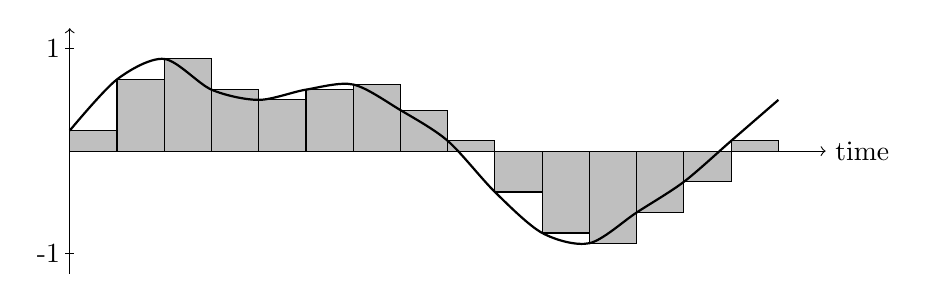
\begin{tikzpicture}[xscale=0.6,yscale=1.3]
  \draw[->] (0,-1.2) -- (0,1.2);
  \draw[->] (0,0) -- (16,0) node[right] {time};
  \draw (-.1,-1) -- (.1,-1);
  \draw (-.1,1) -- (.1,1);
  \draw (0,-1) node[left] {-1};
  \draw (0,1) node[left] {1};
  \r{0}{.2}
  \r{1}{.7}
  \r{2}{.9}
  \r{3}{.6}
  \r{4}{.5}
  \r{5}{.6}
  \r{6}{.65}
  \r{7}{.4}
  \r{8}{.1}
  \r{9}{-.4}
  \r{10}{-.8}
  \r{11}{-.9}
  \r{12}{-.6}
  \r{13}{-.3}
  \r{14}{.1}
  % \r{15}{.5}
  \draw[thick] plot [smooth] coordinates {(0,.2) (1,.7) (2,.9) (3,.6) (4,.5) (5,.6) (6,.65) (7,.4) (8,.1) (9,-.4) (10,-.8) (11,-.9) (12,-.6) (13,-.3) (14,.1) (15,.5)};
\end{tikzpicture}
\end{document}
